\chapter{Evaluation}
\label{chap:eval}

\section{Usability}

First tests and trials have shown that the different approaches are performing differently well. No formal tests and studies have been conducted by now, the following experiences are subjective and by far not representative.

Controlling the hand grasps using the grasp synergy approaches works quite good. The absolute version seems to give the user a little better and direct control about what's actually happening with the hand and thus more dexterity in the grasp operations than the relative approach. Controlling the arm in both approaches, however, is a little inaccurate. While in the absolute approach a small screen is mapped to a relatively large space, the relative approach has it's disadvantages as the gesture activation time takes one second every time a gesture to move the arm is lifted from the screen and the hand is moved to the other edge of the screen and placed down, which affects the workflow significantly, albeit being much more precise. In both approaches, however, the arm does not remain at one stable position when the control gesture is on the screen, but not moved. This results in a noticeable jitter of the arm. The reason for this seems to be the BioIK solver returning different solutions for the same pose. As long as the gesture is active on the screen, new solutions are queried by the application in an endless loop, since the position of the pointers change very little. These changes are in the second to fourth decimal digit of the value of the amplitude, however the BioIK solver returns a new -- and different -- solution for the same position. This effect was dramatically reduced once the \textit{MinimalDisplacementGoals} were added to the request messages, but are still noticeable. Additionally, finding solutions with the \textit{MinimalDisplacementGoal} active in the request takes significantly longer (about factor two, see Section \ref{sec:eval:ikservice}).  These small movements made precise control and positioning of the hand difficult. 

In the direct fingertip mapping, these jitters were even more significant, as the position of the fingertips were to be mapped to positions in space with high dexterity. However, because of the jitter occurring within the BioIK solutions, it is very hard to precisely grasp objects. Again, adding the \textit{MinimumDisplacementGoal} reduced this effect significantly, but slowed down the (already slow) solution finding of BioIK even more.

\section{Performance}

As performance issues occurred during first tests, a small look into where these issues come from shall be given.

\subsection{Application}

The overall performance of the application seems good. No significant lags in response times of the user interface were noticeable. All off-line calculations like calculating joint angles from grasp synergies or fingertip positions in three dimension do not take any significant processing power. While using the application without any inverse kinematic involved, the CPU load was measured well below 5\%. Nonetheless, the device gets significantly warm after a period of usage and the battery power drains perceptibly faster. 

No further effort was done to find out the reason for the warmth and battery drain as it did not directly affect development, but a good assumption might be that the ROS data exchange induces a constant load onto the WiFi chipset of the tablet computer. Joint states are received at about 100 Hz, updates are sent at 10 Hz. Additionally, every BioIK service call issues some wireless communication. This leads to a lot of small packets being sent over the wireless network, resulting in a constant workload preventing the chipset from being put into power saving modes.

\subsection{BioIK Service}
\label{sec:eval:ikservice}

\begin{figure}
	\caption{\label{fig:eval:1000ms}Measurements for 1000ms}
	\begin{center}
		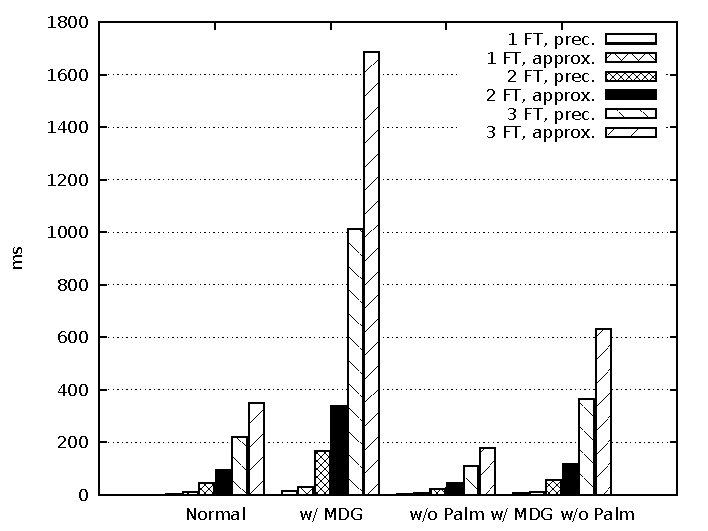
\includegraphics{assets/chpt_eval/1000ms.pdf}
	\end{center}
\end{figure}


It was observed during tests that getting a result from the BioIK service takes significant amounts of time during arm movements controlled by touch gestures and even more time in the direct fingertip mapping mode. In the grasp synergy approaches, an IK request took about 200-300 ms from sending the request until the \textit{onSuccess()} callback was called in the application. This is a frequency of about 5Hz, which is lower than expected but still enaugh for a relatively precise positioning of the arm.

In the direct fingertip mapping approach however, response times varied depending on the number of fingers that were currently mapped, from approx. 600ms when using one finger to about 1.6 seconds with three fingers on the screen. Update frequencies of significantly less than 1 Hz are very disturbing and prevent the application from being used in the desired manner. The time measured is -- again -- the time from calling the service until the \textit{onSuccess()} callback was called. 

Additionally it is observable that when the BioIK service is called, the user interface freezes until a response is processed, resulting in a very juddery user experience. Multiple factors can take effect here:
\begin{itemize}
	\item The rosjava/rosandroid implementation of service calls is faulty. The freezing user interface is an indication for the service calls not being implemented asynchronously as one would think, since a call is initiated with a service response handler which is called when the result was received.
	\item The BioIK service is very slow or has unexpected behaviours.
\end{itemize}

Since debugging of foreign code can be very time-consuming, especially in projects of the size of rosjava and rosandroid, first measurements were done concerning the performance of BioIK. A pose of the robot was chosen which was once returned by the BioIK service, so it's known and sure a solution exists. Then, the following cases were measured:
\begin{itemize}
	\item 1, 2 and 3 fingertips with \textit{approximate = false}.
	\item 1, 2 and 3 fingertips with \textit{approximate = true}.
\end{itemize}

for the following cases:
\begin{itemize}
	\item With OrientationGoal for the palm, without MinimumDisplacementGoal.
	\item Without OrientationGoal for the palm, without MinimumDisplacementGoal.
	\item With OrientationGoal for the palm, with MinimumDisplacementGoal.
	\item Without OrientationGoal for the palm, with MinimumDisplacementGoal.
\end{itemize}

Every test request was executed 200 times, as a result the mean execution time of all calls was taken. The aim was to find out what affects execution time of the BioIK service the most, the suspected properties were the MinimumDisplacementGoal, the additional OrientationGoal for the palm and the \textit{approximate} property of the IK request. Measurements were initially done with a timeout of one second passed to the BioIK solver. A plot of the measurements can be reviewed in Figure \ref{fig:eval:1000ms}. Three interesting things are visible on the first sight:
\begin{itemize}
	\item If the request is marked with \textit{approximate = true}, the solver takes about twice the time as if a precise solution is requested.
	\item The \textit{MinimumDisplacementGoal} seems to have a huge effect on execution time, multiplying the time by a factor of about 4-5.
	\item The time needed by the solver is highly dependent on the number of fingertips included in the request. 
\end{itemize}

\begin{figure}
	\caption{\label{fig:eval:10ms}Measurements for 10ms}
	\begin{center}
		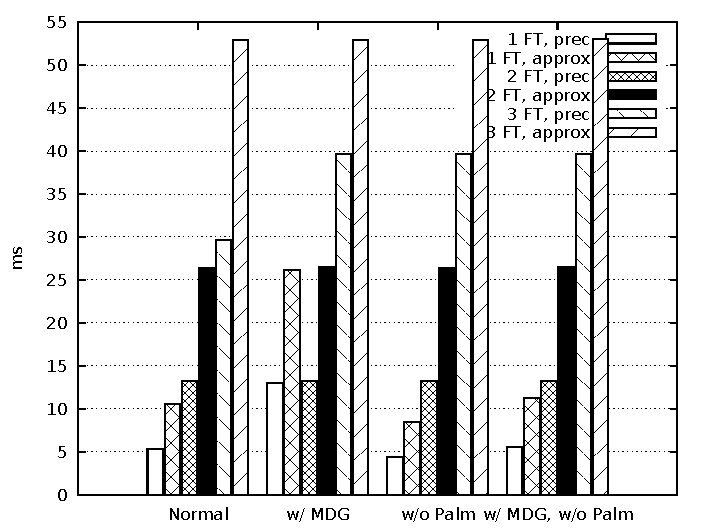
\includegraphics{assets/chpt_eval/10ms.pdf}
	\end{center}
\end{figure}

All tests were repeated setting the \textit{timeout} for the request to 10 ms. The test results are represented in Figure \ref{fig:eval:10ms}. Surprisingly this rendered all measurements completely different. Execution times are nearly constant for every fingertip configuration, the dependency seems to be exponential. The only real difference visible is the measurement of one fingertip with \textit{OrientationGoal} for the Palm and with \textit{MinimumDisplacementGoal}, which is about factor three bigger than without the \textit{MinimumDisplacementGoal}. Most importantly, the maximum times of about 55ms were about two orders of magnitude smaller than the maximum values measured with a timeout of one second. The execution time of the BioIK solver seems to be dependent on the timeout it is passed, using more time when the timeout is bigger. This assumption was confirmed by \citeauthor{Ruppel17}\cite{Ruppel17} who states that the BioIK solver \textbf{can} return a result before the timeout is exceeded, but does not necessarily do so.

As a consequence, a time-out of 10ms was set for the BioIK service calls within the Android application. The results, again, were surprising, as no significant improvement was observed. The only difference then was that the BioIK solver returned an error code indicating no solution was found, increasing the timeout up to 500ms rendered the DFTM approach usable again, but still with response times of 1.2 to 1.6 seconds. At the time of writing open questions remain. It is yet to be found out why the service calls take such a long time in rosjava/rosandroid, rendering the user interface frozen with the response time not significantly impacted by the timeout set in the request.

\section{Possible User Studies}

With user studies, it could be found out how well the different approaches implemented here work with untrained and trained test persons. Data can be recorded either objectively by measuring times and judging how successful the execution of a task has been or subjectively, by asking the user about how difficult or easy the task for was him. A famous, standardized questionnaire is the NASA TLX (Task Load Index) test\cite{Hart1988}. It gives a good insight of how stressful a task was for the user. Besides these standardized tests, a domain-specific test should be developed to get data about the actual environment that shall be evaluated.

Each test person should perform multiple tasks with a rising level of difficulty. For example:
\begin{itemize}
	\item Grasp an object and release it.
	\item Grasp an object, move it to another place and release it.
	\item Grasp an object, put it into a box placed nearby.
\end{itemize}
These tasks can then be performed for both multiple objects (balls, cylinders, cuboids) of different materials (sponge, wood, rubber) and the three different approaches. Each task shall be completed multiple times, while the time needed to complete the task is measured. This gives an insight in how fast a specific task can be trained. Additionally, after the task was executed multiple times by one user, he shall be queried for how difficult he thinks the task was, how much help he needed and how intuitive he thinks the control was. The test supervisor shall also note how much help he had to give to the test person to give an insight on how different perception was. 

From the data raised during these studies a conclusion can be made which approach is probably the best to grasp a variety of objects, which is the easiest to learn, which one is the most intuitive and which one causes the least stress on the operator. These results could then be used in further development and improvement of tele-manipulation methods using a decterous robotic hand and a robot arm, combined to a robot system with a high number of degrees-of-freedom.